\documentclass{article}

\usepackage{amsmath}
\usepackage{amssymb}
\usepackage{amsfonts}
\usepackage{mathtools}

\usepackage[thmmarks, amsmath]{ntheorem}

\usepackage{graphicx}
\usepackage{fullpage}
\usepackage{tikz-cd}
\usepackage{tikz}
\usepackage{float}

\usepackage{diffcoeff}
\diffdef{}{op-symbol=\mathrm{d},op-order-sep=0mu}

\usepackage{cancel}

\usepackage{enumitem}

\setlist[enumerate,1]{label=\alph*)}

\title{Notes on Ordinals}
\author{Duarte Maia}
%\date{}

\theorembodyfont{\upshape}
\theoremseparator{.}
\newtheorem{theorem}{Theorem}
\newtheorem{prop}{Proposition}
\renewtheorem*{prop*}{Proposition}
\newtheorem{lemma}{Lemma}
\newtheorem{definition}{Definition}

\theoremstyle{nonumberplain}
\newtheorem{convention}{Convention}

\theoremheaderfont{\itshape}
\theorembodyfont{\upshape}
\theoremseparator{:}
\theoremsymbol{\ensuremath{\blacksquare}}
\newtheorem{proof}{Proof}
\theoremsymbol{\ensuremath{\square}}
\newtheorem{proofsketch}{Proof Sketch}

\theoremsymbol{\ensuremath{\square}}
\newtheorem{sketch}{Proof Sketch}

\newcommand{\N}{\mathbb{N}}
\newcommand{\Z}{\mathbb{Z}}
\newcommand{\Q}{\mathbb{Q}}
\newcommand{\R}{\mathbb{R}}
\newcommand{\C}{\mathbb{C}}

\DeclarePairedDelimiter{\braket}{\langle}{\rangle}

\newcommand{\below}[1]{{#1\!\!\downarrow}}


\begin{document}
\maketitle

\section{Introduction}

This document is just some notes I'm keeping for myself to keep track of what I've proved regarding ordinals.

\section{Groundwork}

\begin{definition}
An ordinal is the order type of a well-ordered set.
\end{definition}

The endgoal of this section is to show that any ordinal has a canonical representative, which is something called an $N$-set (see below). Moreover, if we identify each ordinal with this canonical representative, we collect an assortment of useful properties and constructions.

\begin{definition}
A set $X$ is said to be transitive if $x \in y \in X$ implies $x \in X$. If $X$ and all its elements are transitive, the relation $(\in) \subseteq X \times X$ is transitive, and assuming some kind of foundation axiom, is nonreflexive and antisymmetric, thereby forming a partial order on $X$.

We say that a transitive set $X$ is an $N$-set if the order given by $\in$ is a well-ordering of $X$.
\end{definition}

\begin{theorem}
If $X$ is any well-ordered set, it is order-isomorphic to an $N$-set.
\end{theorem}

\begin{proofsketch}
First, we show that, for all $x \in X$, the set $\below x = \{y \in X \mid y\leq x\}$ is isomorphic to an $N$-set. Indeed, since $X$ is well-ordered, supposing that there is some $x$ such that $\below x$ is not isomorphic to an $N$-set, we may pick a minimal one.

For each $y < x$, define $N(y)$ as an $N$-set which is isomorphic to $\below y$. This step is mildly sketchy, but will be less so once we show that $N(y)$ is actually unique. Now, we set $Z =\bigcup_{y<x} N(y)$, which by proposition \ref{prop:w} is itself an $N$-set, and that $Z \cup \{Z\}$ is isomorphic to $\below x$. The basic idea is that the isomorphisms between $\below y$ and $N(y)$ as $y$ ranges over $X_{<x}$ are compatible, in the sense that if $y < y'$ then $N(y) \subseteq N(y')$ and moreover the following diagram commutes:
\begin{equation}
\begin{tikzcd}
\below y \arrow[d, "\cong" ] \arrow[r, hook] & \below{y'} \arrow[d, "\cong" ] \\
N(y) \arrow[r, hook]                                    & N(y')                                    
\end{tikzcd}
\end{equation}

As such, the isomorphisms can be glued together to yield an order isomorphism between $\bigcup_{y<x} \below y$ and $Z = \bigcup_{y<x} N(y)$, which we extend to $\below x$ by sending $x$ to $Z \in Z \cup \{Z\}$. See also proposition \ref{prop:suc} to see that $Z \cup \{Z\}$ is itself an $N$-set, and in fact order isomorphic to $Z+1$.

Now that we've shown that all $\below x$ are isomorphic to a unique $N(x)$, it suffices to reproduce the same argument to conclude that $\bigcup_{x \in X} \below x$ is isomorphic to $W = \bigcup_{x\in X} N(x)$, which is itself an $N$-set, and the proof is complete.
\end{proofsketch}

Now we go back and prove the propositions we need to make the proof work. It should be noted that two of the steps are extremely similar in character, so we group them into a single proposition. Define
\begin{equation}
W = \bigcup_{y \in X_0} N(y),
\end{equation}
where $X_0$ is an initial segment of $X$. We will show that this is order isomorphic to $X_0$. We apply this to the following two cases:
\begin{itemize}
\item For $X_0 = (\below x)\setminus \{x\}$, to show that if for all $y < x$ there is some $N(y)$ then there is some $N(x)$,
\item For $X_0 = X$, to show that if for all $x$ there is some $N(x)$ then there is an $N$-set which is isomorphic to $X$.
\end{itemize}

So we boil the proof down to the following lemma.

\begin{prop}
Let $X_0$ be a well-ordered set such that each $x \in X_0$ satisfies $\below x \cong N(x)$ for some $N$-set $N(x)$. Then, $X_0$ is isomorphic to $W = \bigcup_{x \in X_0} N(x)$, which is an $N$-set.
\end{prop}

\begin{proof}
First, we claim that $W$ is indeed an $N$-set (proposition \ref{prop:w} below). Moreover, by proposition \ref{prop:nat} below, the maps $\below x \to N(x) \hookrightarrow W$ agree where mutually defined, and so can be glued to yield a well-defined map $X_0 \to W$. Since this is a gluing of monotone functions, defined on initial segments of $X_0$, the resulting map is still monotone, and hence injective. Finally, since $W$ is, by definition, the union of the images of the functions being glued, the glued function is also surjective. Thus, it is an isomorphism and the proof is complete.
\end{proof}

\begin{prop}\label{prop:w}
Let $W = \{N_\alpha\}_{\alpha \in A}$ be a collection of $N$-sets. Then, $W = \bigcup N_\alpha$ is an $N$-set.
\end{prop}

\begin{proof}
\leavevmode
\begin{itemize}
\item Transitivity: If $x \in y \in W$ then $x \in y \in N_\alpha$ for some $\alpha$, thus $x \in N_\alpha \subseteq W$.
\item $(\in)$ is transitive: If $x \in y \in z \in W$ then these three lie in some common $N_\alpha$ and the result follows.
\item $(\in)$ satisfies trichotomy: Let $x, y \in W$. Then (see prop \ref{prop:tri} below) $x$ and $y$ are in some common $N$-set, and so trichotomy holds.
\item $(\in)$ is a well-order: Let $S \subseteq W$ be nonempty. Given an element $x \in S$, consider $S_0 = S \cap N_\alpha$, where $x \in N_\alpha$. Then, $S_0 \neq \emptyset$ and has a minimum $m$, so it suffices to show that $m$ is in fact a minimum of $S$.

Given $s \in S$, either $s \in N_\alpha$, in which case $m \in s$, or $s \in N_\beta \setminus N_\alpha$ for some $\beta$, and by proposition \ref{prop:tri} below we have $m \in N_\alpha \in s$, hence by transitivity $m \in s$. The proof is complete.
\end{itemize}
\end{proof}


\begin{prop}\label{prop:tri}
If $A$ and $B$ are two $N$-sets, either $A \in B$, $B \in A$, or $A = B$.

In particular, either $A \subseteq B$ or $B \subseteq A$.

Moreover, if $s \in B \setminus A$ we have $B \nsubseteq A$, hence $A \in B$, and since $s \notin A$ we have $A \in s$.
\end{prop}

\begin{proof}
To begin this proof, it is useful to point out that $A \cap B$ is an initial segment of both $A$ and $B$, by transitivity. Thus, the picture to have in mind is one like this:

\begin{figure}[H]
\centering
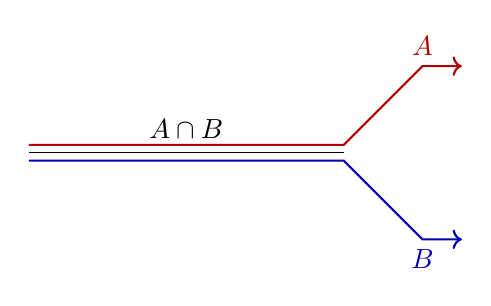
\begin{tikzpicture}
\draw (0,0) -- (4,0) node[midway,above=0.4ex] {$A \cap B$};
\draw[red!70!black, ->, thick] (0,0.1) -- ++(4,0) -- ++(1,1)node[above]{$A$} --++(0.5,0);
\draw[blue!70!black, ->, thick] (0,-0.1) -- ++(4,0) -- ++(1,-1)node[below]{$B$} --++(0.5,0);
\end{tikzpicture}
\end{figure}

Now, the way forward is as follows. Pick a minimal element $a$ of $A \setminus B$, and a minimal element $b$ of $B \setminus A$, if neither is empty. In this case, we will show that they must both be
\begin{equation}\label{eq:abab}
a = b = A \cap B,
\end{equation}
which contradicts the definitions of $a$ and $b$. Thus, they will not both be able to exist and either $A \subseteq B$ or vice versa.

We will in fact be able to obtain more detail. For example, if $a$ exists, then $b$ cannot, hence $B = A \cap B = a \in A$, and thus $B \in A$. Likewise, if $b$ exists then $A \in B$, and the only missing case, where neither exists, is the one where $A = B$, and thus we obtain the trichotomy  in the proposition. The only remaining step is to prove \eqref{eq:abab}, which we leave as its own proposition.
\end{proof}

\begin{prop}
Let $A$ be an $N$-set, and $A_0$ a strict subset of $A$, which is also an initial segment. Let $a \in A \setminus A_0$ be minimal. Then, $a = A_0$.
\end{prop}

\begin{proof}
First, we show that $A_0 \subseteq a$. To do so, pick $x \in A_0$. Then, since $A_0$ is an initial segment, $x \in a$. (Otherwise, either $a = x \in A_0$, contradiction, or $a \in x \in A_0$, which by def. initial segment implies $a \in A_0$, contradiction.) This proves $A_0 \subseteq a$.

To show the other inclusion, we refer to proposition \ref{prop:leq} below, which shows that either $A_0 = a$ (as desired) or $A_0 \in a$. But if the latter is the case, then $A_0 \in A$, but since $A_0 \notin A_0$ we get $A_0 \in A \setminus A_0$ yet $A_0 \in a$, contradicting the minimality of $a$.
\end{proof}

\begin{prop}\label{prop:leq}
If $X$ is an $N$-set and $x,y \in X$, then $x \subseteq y$ iff $x \in y$ or $x = y$. In other words, $\subseteq$ is to $\in$ as $\leq$ is to $<$.
\end{prop}

\begin{proof}
$(\leftarrow)$ is obvious by transitivity, so we focus on showing $(\rightarrow)$.

Suppose that neither $x \in y$ nor $x = y$. Then, since $X$ is totally ordered by membership, we have that $y \in x$. Thus, $y$ is an element of $x$ which is not an element of $y$, hence $x \nsubseteq y$.
\end{proof}

In the course of proving proposition \ref{prop:tri} we obtain a little bit of extra specificity which will be useful.

\begin{prop}
If $X$ and $Y$ are two $N$-sets, one is contained in the other as an initial segment.
\end{prop}

\begin{prop}\label{prop:nat}
Let $A_0$ be an initial segment of $A$, and $B_0$ an initial segment of $B$. Moreover, pick isomorphisms $f \colon A_0 \cong B_0$ and $g \colon A \cong B$. Then, the following diagram commutes.
\begin{equation}
\begin{tikzcd}
A_0 \arrow[d, "\cong" ] \arrow[r, hook] & A \arrow[d, "\cong" ] \\
B_0 \arrow[r, hook]                                    & B
\end{tikzcd}
\end{equation}

In particular, if $A_0 = A$ and $B_0 = B$, we conclude that an isomorphism between well-ordered sets, if it exists, is unique.
\end{prop}

\begin{proof}
What we want to show effectively amounts to proving that $f = g|_{A_0}$. In other words, for all $x \in A_0$ we have $f(x) = g(x)$. As such, we suppose that this is not the case, and pick a minimal value of $x \in A_0$ such that $f(x) \neq g(x)$. We will obtain a contradiction, by showing that both $f(x)$ and $g(x)$ are (uniquely) determined by the expression
\begin{equation}\label{eq:fgb}
f(x) = g(x) = \min B \setminus \{f(z) \mid z < x\}.
\end{equation}

We prove the slightly more general statement: if $f \colon A_0 \to B_0$ is an isomorphism of well-ordered sets, for any $x \in A_0$ we have that $f(x)$ is the minimal element which is stricty greater than $f(z)$ for all $z < x$. Equation \eqref{eq:fgb} follows because $B_0$ is an initial segment of $B$.

Now, by monotony, we definitely have that $f(x) > f(z)$ whenever $z < x$. However, suppose that $f(x)$ was not the minimal element in these conditions. Then, there would be some $f(z) < b < f(x)$. But $b = f(k)$ for some value of $k \in X$ with $z < k < x$, which shows that $b$ is not greater than $f(z)$ for all $z < x$, namely for $z = k$.
\end{proof}

\begin{prop}\label{prop:suc}
If $Z$ is an $N$-set, $Z \cup \{Z\}$ is an $N$-set, and it is order isomorphic to $Z+1$.
\end{prop}

\begin{proof}
\leavevmode
\begin{itemize}
\item Transitivity is obvious.
\item To show the other properties, it suffices to notice that indeed the $(\in)$ relation on $Z \cup \{Z\}$ behaves like the order in $Z+1$, so the same proof that shows that $Z+1$ is a well-ordered set also functions here.
\end{itemize}
\end{proof}

\end{document}